\section{Flächenträgheitsmomente}
    \begin{center}
        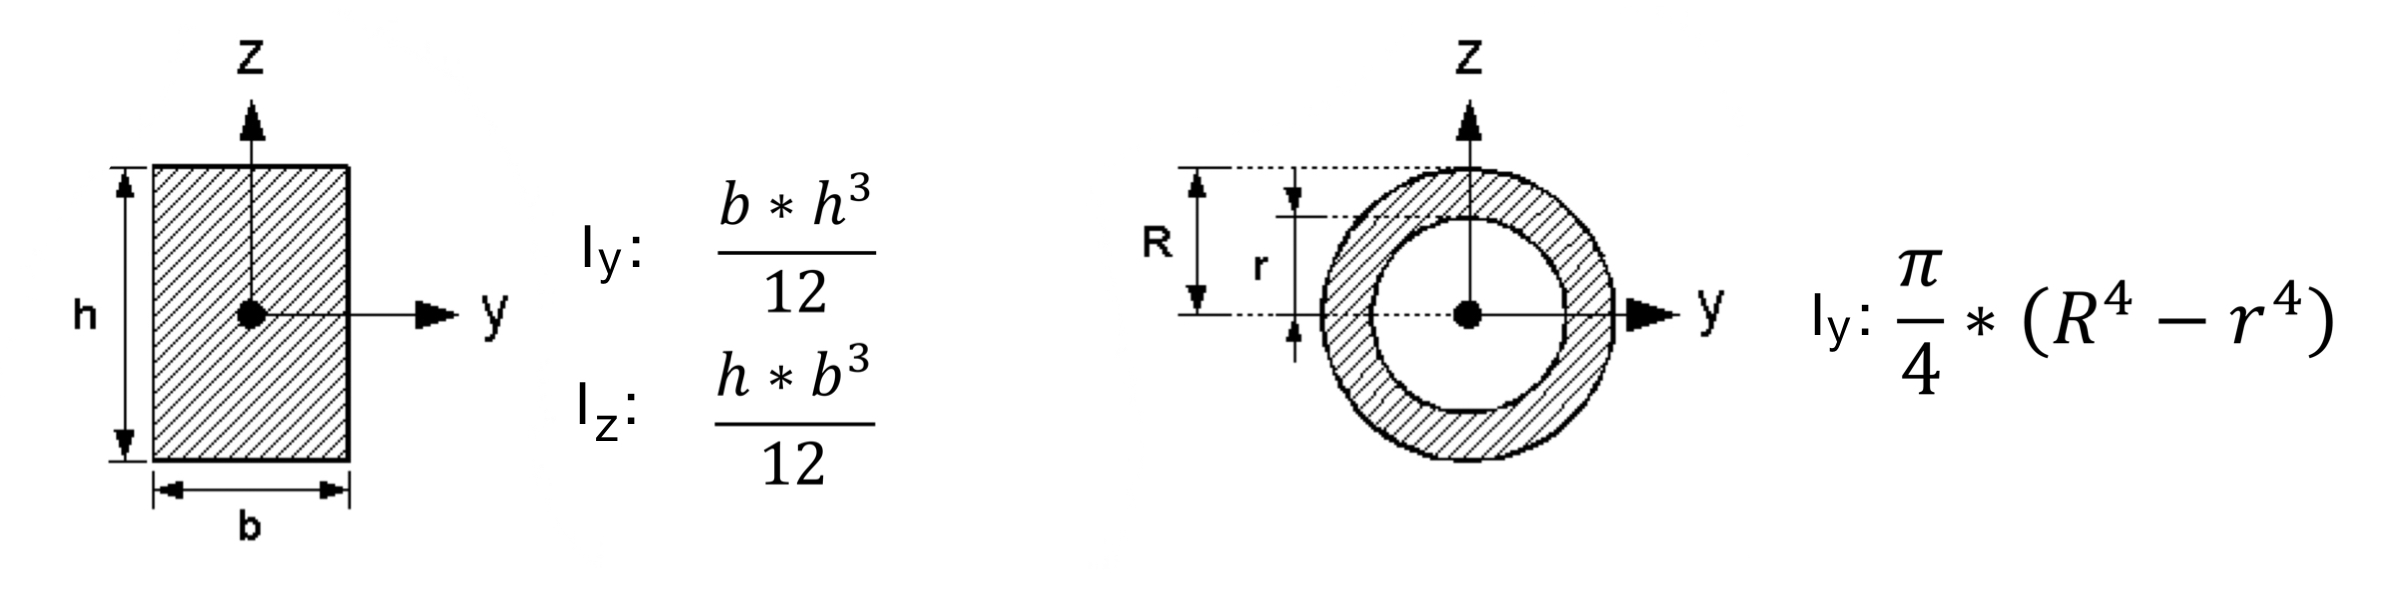
\includegraphics[width= 0.8\linewidth]{10/traegheitsmom.jpeg}
    \end{center}
\section{Kesselgleichungen}
    Für \textbf{geschlossene}, dünnwandige Behälter ($\frac{d}{R} \ll 1$):
    \[\sigma_{\varphi\varphi} = \frac{R}{d}P = 2\sigma_{zz}; \quad \sigma_{zz} = \frac{R}{2d}P \textrm{ }(\textrm{offen: }\sigma_{zz}=0); \quad \sigma_{rr}=0\]
    Für dünnwandige, \textbf{kugelförmige} Behälter:
    \[\sigma_{\varphi\varphi}=\sigma_{\theta\theta}=\frac{R}{2d}P; \quad \sigma_{rr}=0\]


